\icode{N14W-MCC-SI-L3-261025-001}
\nceeID[6]{2014安徽}{19}
如图所示，一倾斜的匀质圆盘绕垂直于盘面的固定对称轴以恒定角速度\(\omega\)转动，盘面上离转轴距离\qty{2.5}{m}处有一小物体与圆盘始终保持相对静止，物体与盘面间的动摩擦因数为\(\frac{\sqrt{3}}{2}\)，（设最大静摩擦力等于滑动摩擦力），盘面与水平面的夹角为\qty{30}{\degree}，\(g\)取\qty{10}{m/s^2}，则\(\omega\)的最大值是\paren[]
	
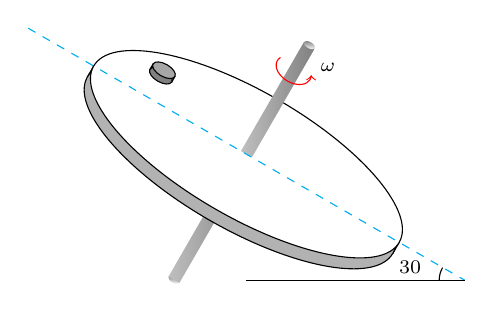
\begin{tikzpicture}[scale=.8,font=\scriptsize]
	\begin{scope}[rotate=-30]
		\shade[gray] (0,-2.3) ellipse(.1 and .05);
		\shade[left color=gray!50!white,right color=gray] (-.1,0) rectangle(0.1,-2.3);
		\draw[fill=gray!70] (-2.8,.-.2) rectangle(2.8,0);
		\draw[fill=gray!60] (0,-.2) ellipse(2.8 and 1);
		\draw[fill=white] (0,0) ellipse(2.8 and 1);
		\shade[left color=gray!50!white,right color=gray] (-.1,2) rectangle(.1,0);
		\shade[gray] (0,2) ellipse(.1 and .05);
		\draw[dashed,cyan] (-4,0)--(4,0);
		\draw[->,red] (-.3,1.6) arc(-200:20:.3 and .2);
		\draw[fill=gray] (-2,.4) rectangle(-1.6,.5);
		\draw[fill=gray] (-1.8,.4) ellipse(.2 and .1);
		\draw[fill=gray!70] (-1.8,.5) ellipse(.2 and .1);
		\node at(.2,1.7)[right]{\(\omega\)};
	\end{scope}
	\draw[yshift=-2cm] (0,0)--({2*sqrt(3)},0);
	\draw[yshift=-2cm,xshift=3.46cm] (-.4,0) arc(180:150:.4);
	\node at(2.6,-1.8){\qty{30}{\degree}};
\end{tikzpicture}
\begin{choices}
	\item \(\sqrt{5}\)\qty{}{rad/s}
	\item \(\sqrt{3}\)\qty{}{rad/s}
	\item \qty{1.0}{rad/s}
	\item \qty{0.5}{rad/s}
\end{choices}
\begin{answer}

\end{answer}